%
% File naaclhlt2016.tex
%

\documentclass[11pt,letterpaper]{article}
\usepackage{naaclhlt2016}
\usepackage{times}
\usepackage{latexsym}
\usepackage{graphicx}
\usepackage{subcaption}
\usepackage{tabularx}

\naaclfinalcopy % Uncomment this line for the final submission
\def\naaclpaperid{***} %  Enter the naacl Paper ID here

% To expand the titlebox for more authors, uncomment
% below and set accordingly.
% \addtolength\titlebox{.5in}    

\newcommand\BibTeX{B{\sc ib}\TeX}


\title{Crowdsourcing for (almost) Real-time Question Answering}

% Author information can be set in various styles:
% For several authors from the same institution:
% \author{Author 1 \and ... \and Author n \\
%         Address line \\ ... \\ Address line}
% if the names do not fit well on one line use
%         Author 1 \\ {\bf Author 2} \\ ... \\ {\bf Author n} \\
% For authors from different institutions:
% \author{Author 1 \\ Address line \\  ... \\ Address line
%         \And  ... \And
%         Author n \\ Address line \\ ... \\ Address line}
% To start a seperate ``row'' of authors use \AND, as in
% \author{Author 1 \\ Address line \\  ... \\ Address line
%         \AND
%         Author 2 \\ Address line \\ ... \\ Address line \And
%         Author 3 \\ Address line \\ ... \\ Address line}
% If the title and author information does not fit in the area allocated,
% place \setlength\titlebox{<new height>} right after
% at the top, where <new height> can be something larger than 2.25in

\author{Denis Savenkov \\ Emory University \\ {\tt dsavenk@emory.edu} 
  \And Scott Weitzner \\ Emory University \\ {\tt sweitzn@emory.edu}
  \And Eugene Agichtein \\ Emory University \\ {\tt eugene@mathcs.emory.edu}
}

\date{}

\begin{document}

\maketitle

\begin{abstract}

Modern search engines have made dramatic progress in the answering of many user's questions about facts, such as those that might be retrieved or directly inferred from a knowledge base.
However, many other questions that real users ask are more complex, such as asking for opinions or advice for a particular situation, and are still largely beyond the competence of the computer systems.
As conversational agents become more popular, QA systems are increasingly expected to handle such complex questions, and to do so in (nearly) real-time, as the searcher is unlikely to wait longer than a minute or two for an answer.
One way to overcome some of the challenges in complex question answering is crowdsourcing.
We explore two ways crowdsourcing can assist a question answering system that operates in (near) real time: by providing answer validation, which could be used to filter or re-rank the candidate answers, and by creating the answer candidates directly.
Specifically, we focus on understanding the effects of time restrictions in the near real-time QA setting.
Our experiments show that even within a one minute time limit, crowd workers can produce reliable ratings for up to three answer candidates, and generate answers that are better than an average automated system from the LiveQA 2015 shared task.
Our findings can be useful for developing hybrid human-computer systems for automatic question answering and conversational agents.

\end{abstract}

\section{Introduction}
\label{sec:introduction}

It has long been a dream to communicate with a computer as one might with another human being using natural language speech and text.
Nowadays, we are coming closer to this dream, as natural language interfaces become increasingly popular.
Our phones are already reasonably good at recognizing speech, and personal assistants, such as Apple Siri, Google Now, Microsoft Cortana, Amazon Alexa, etc., help us with everyday tasks and answer some of our questions.
Chat bots are arguably considered ``the next big thing'', and a number of startups developing this kind of technology has emerged in Silicon Valley and around the world\footnote{http://time.com/4194063/chatbots-facebook-messenger-kik-wechat/}.

Question answering is one of the major components of such personal assistants.
Existing techniques already allow users to get direct answers to their factoid questions.
%\footnote{https://www.stonetemple.com/rich-answers-in-search/}.
However, there is still a large number of more complex questions, such as advice or accepted general opinions, for which users have to dig into the ``10 blue links'' and extract or synthesize answers from information buried within the retrieved documents.
To cater to these informational needs, community question answering (CQA) sites emerged, such as Yahoo! Answers and Stack Exchange.
These sites provide a popular way to connect information seekers with answerers.
Unfortunately, it can take minutes or hours, and sometimes days, for the community to respond, and some questions are left unanswered altogether. 

To facilitate research on this challenge, TREC LiveQA shared task\footnote{www.trec-liveqa.org} was started in 2015, where automated systems attempt to answer real users' questions within a 1 minute period.
This task was successful, with the winning system able to automatically return a reasonable answer to more than half of the submitted questions, as assessed for TREC by the trained judges from NIST.
Nevertheless, many questions were unable to be answered well by any of the participating systems.

In this work we explore two ways common crowdsourcing can be used to help an automated system answer complex user questions in near real-time scenario, e.g., within a minute.
More specifically, we study if crowd workers can quickly and reliably judge the quality of the proposed answer candidates, and if it is possible to obtain reasonable written answers from the crowd within a limited amount of time.
Our research questions can be stated as:
\vspace{-0.3cm}
\begin{enumerate}
\setlength{\itemsep}{0pt}
\setlength{\parskip}{0pt}
\item RQ1. Can crowdsourcing be used to judge the quality of answers to non-factoid questions under a time limit?
\item RQ2. Is it possible to use crowdsourcing to collect answers to real user questions under a time limit?
\item RQ3. How does the quality of crowdsourced answers to non-factoid questions compare to original CQA answers, and to automatic answers from TREC LiveQA systems?
\end{enumerate}


\section{Methodology}
\label{sec:methodology}

To answer the research questions, we conducted a series of crowdsourcing experiments using the Amazon Mechanical Turk platform\footnote{http://mturk.com}.
We used questions from the TREC LiveQA 2015 shared task, along with the system answers, rated by the NIST assessors\footnote{https://sites.google.com/site/trecliveqa2016/liveqa-qrels-2015}.
The questions for the task were selected by the organizers from the live stream of questions posted to the Yahoo! Answers CQA platform on the day of the challenge (August 31, 2015).
For these questions we also crawled their community answers, that were eventually posted on Yahoo! Answers\footnote{As the answer we took the top question, which was selected as the ``Best answer'' by the author of the question or by the community.}.

To check if crowdsourcing can be used to judge the quality of answers under a time limit (RQ1), we asked workers to rate answers to a sample of 100 questions using the official TREC rating scale:
\vspace{-0.3cm}
\begin{enumerate}
\setlength{\itemsep}{0pt}
\setlength{\parskip}{0pt}
\item Bad - contains no useful information
\item Fair - marginally useful information
\item Good - partially answers the question
\item Excellent - fully answers the question
\end{enumerate}

\begin{figure}[h!]
\centering
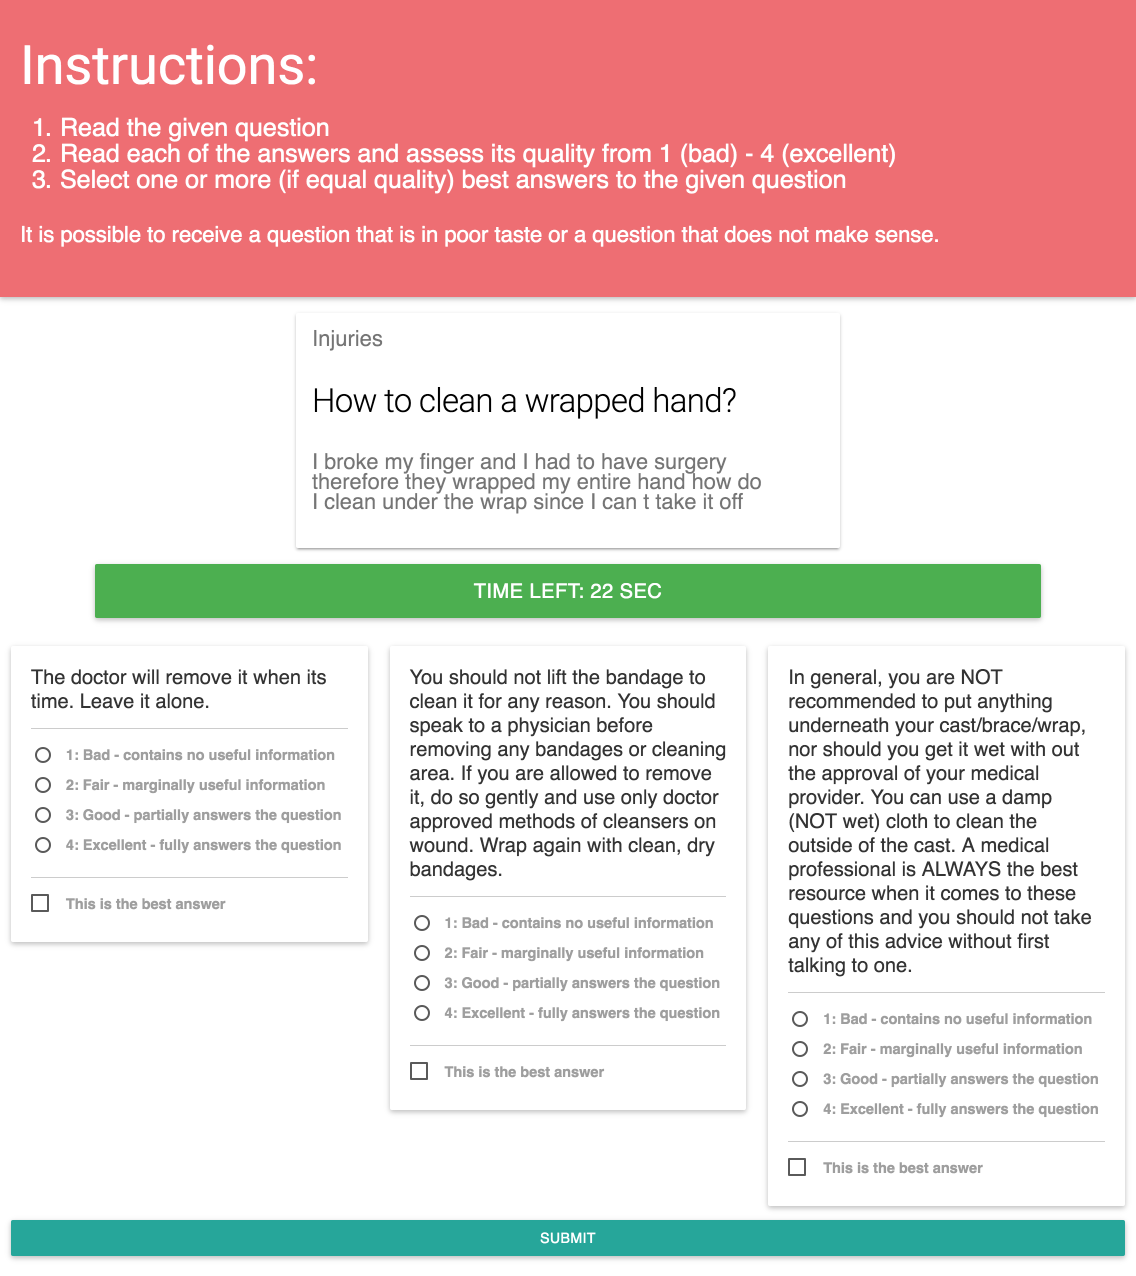
\includegraphics[width=0.9\linewidth]{img/validation_screenshot}
\caption{Answer validation form}
\label{fig:interfaces:validation}
\end{figure}

\begin{figure}[h!]
\centering
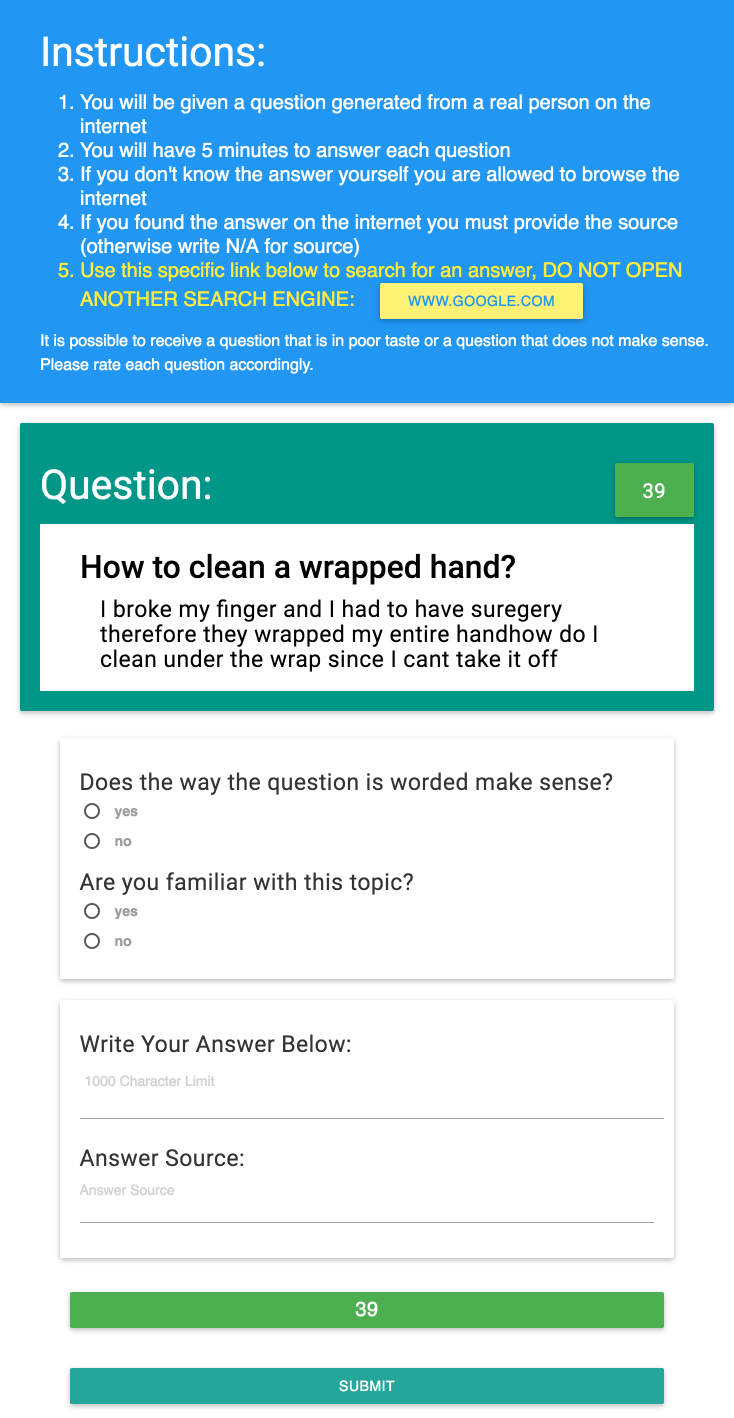
\includegraphics[width=0.75\linewidth]{img/answering_screenshot2}
\caption{Answer crowdsourcing form}
\label{fig:interfaces:answer}
\vspace{-7mm}
\end{figure}


We chose to display 3 answers for a question, which were generated by three of the top-10 automatic systems from TREC LiveQA 2015 evaluation \cite{overviewliveqa15}.
To study the effect of time pressure on the quality of judgments we split participants into two groups. One group made their assessments with a 1 minute countdown timer shown to them, while the other could complete the task without worrying about a time limit.
Within each group, we assigned three different workers per question, and the workers were compensated at a rate of \$0.05 per question for this task.

The interface for collecting answer ratings is illustrated in Figure \ref{fig:interfaces:validation}\footnote{The screenshots show the final state of the form, as we describe later in this sections fields were unhidden step-by-step for proper timing of reading, answering and validation}.
On top of the interface workers were shown the instructions on the task, and question and answers were hidden at this time.
They were instructed to read the question, read the answers, and rate each answer's quality on a scale from 1 (Bad) to 4 (Excellent), and finally choose a subset of candidates that best answer the question.
Upon clicking a button to indicate that they were done reading the instructions, the question, a 60 second countdown timer and 3 answers to the question appeared on the screen.
At the 15 second mark the timer color changed from green to red.
In the experiments without time pressure the timer was hidden, but we still tracked the time it took for the workers to complete the task.

In another experiment, designed to answer RQ2 and check whether crowd workers can provide an answer to a given question within a limited amount of time, we asked different workers to answer the questions from TREC LiveQA 2015.
We split the workers into two groups and displayed a one minute countdown timer for one of them.
We left a grace period and let the workers submit their answers after the timer had run out.
The workers received a \$0.10 compensation for each answer.
The form for answer crowdsourcing is shown in Figure \ref{fig:interfaces:answer}, and similar to the answer rating form, it starts with a set of instructions for the task.
We let the users browse the internet if they were not familiar with the topic or could not answer the question themselves.
To prevent them from finding the original question on Yahoo! Answers, we included a link to Google search engine with a date filter enabled\footnote{https://www.google.com/webhp?tbs=cdr:1,cd\_max:8/30/2015}.
Using this link, workers could search the web as it was on 8/30/2015, before TREC LiveQA 2015 questions were posted and therefore workers were in the same conditions as automatic systems on the day of challenge\footnote{The ranking of search results could be different on the day of the challenge and for our workers}.
Initially, the question was hidden for proper accounting of question-reading and answering times.
Upon clicking a button to indicate that they were done reading the instructions, a question appeared along with a button, which needed to be clicked to indicate that they were done reading the question.
After that, the answering form appears, it contained four fields:
\vspace{-0.4cm}
\begin{enumerate}
\setlength{\itemsep}{0pt}
\setlength{\parskip}{0pt}
\item Does the question make sense: ``yes'' or ``no'' to see if the question was comprehensible
\item Are you familiar with the topic: A yes or no question to evaluate whether the worker has had prior knowledge regarding the question topic
\item Answer: the field to be used for the user's answer to the given question
\item Source: the source used to find the answer: URL of a webpage or NA if the worker used his own expertise
\end{enumerate}

\vspace{-0.4cm}
Finally, to compare the quality of the collected answers with automatic system and CQA responses (RQ3) we pooled together the crowdsourced answers, the answers from the winning and other top-10 LiveQA'15 systems, and the original answers crawled from Yahoo! Answers.
Each set of answers was given to mechanical turk workers for ratings.


\section{Results and Discussion}
\label{sec:results}

In this section we will describe our results and discuss some of the implications.
We start from the results on answer rating (Section \ref{subsec:results:answer_rating}), and then describe the answer crowdsourcing experiment (Section \ref{subsec:results:answer_crowd}).

\subsection{Answer rating}
\label{subsec:results:answer_rating}

In the answer rating experiment we collected 6 ratings (3 with and 3 without time pressure) for each of three answers for a sample of 100 questions, which makes it a total of 1800 judgments.
Each answer also has an official NIST assessor rating on the same scale.
Figure \ref{figure:score_correlation} shows correlation between official NIST assessor relevance judgments and ratings provided by our workers.
The Pearson correlation between the scores is $\rho=0.52$.
The distribution of scores shows that official assessors were very strict and assigned many extreme scores of 1 or 4, whereas mechanical turk workers preferred intermediate 2s and 3s.
The results did not show any significant differences between experiments with and without time pressure.
Figure \ref{figure:validation_time} shows that even though the median time to rate all three answers is around 22-25 seconds in both experiments, the upper bound is significantly lower in the experiment with the time pressure.

\begin{figure}[t!]
	\centering
	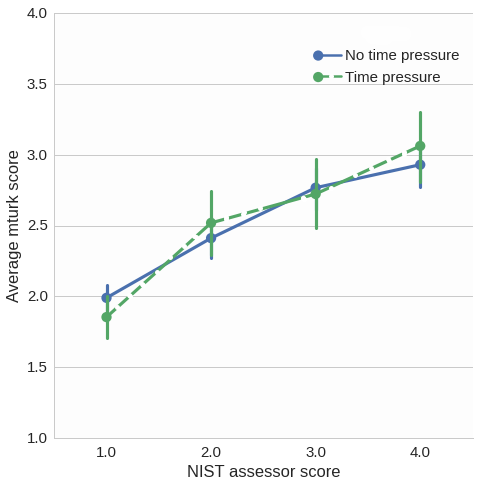
\includegraphics[width=0.35\textwidth]{img/score_correlation}
	\caption{Correlation between NIST assessor scores and crowdsourced ratings with and without time limit on the work time}
	\label{figure:score_correlation}
\end{figure}

\begin{figure}[t!]
	\centering
	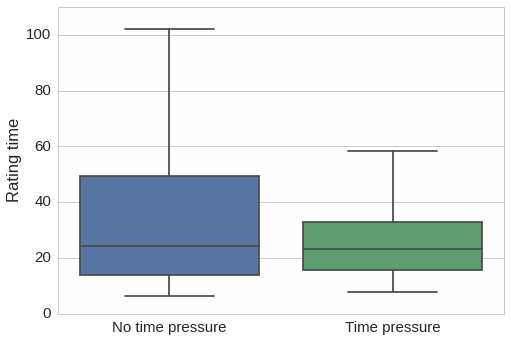
\includegraphics[width=0.4\textwidth]{img/validation_time}
	\caption{Box plot of answer rating time with and without time pressure}
	\label{figure:validation_time}
\end{figure}


Therefore, we conclude that in general we can trust crowdsourced ratings, and on average one minute is enough to judge the quality of three answers to CQA questions.

\subsection{Answer crowdsourcing}
\label{subsec:results:answer_crowd}

In the answer crowdsourcing experiment we collected 6 answers (3 with and without time pressure) for each of the 1087 LiveQA'15 questions.
Since we have answers from different sources, let's introduce the following notations:
\vspace{-0.25cm}
\begin{itemize}
\setlength{\itemsep}{0pt}
\setlength{\parskip}{0pt}
	\item \textit{Yahoo! Answers} - answers eventually posted by users on Yahoo! Answers for the original questions
	\item \textit{Crowd} - answers collected from Mechanical Turk workers without time pressure
	\item \textit{Crowd-time} - answers collected from Mechanical Turk workers with one minute time pressure
	\item \textit{LiveQA winner} - answers from the TREC LiveQA'15 winning system
	\item \textit{LiveQA top10} - answers from another top 10 TREC LiveQA'15 system.
\end{itemize}
\vspace{-0.3cm}	

%\footnote{We will release the data for the community???}.
Table \ref{table:answer_stats} summarizes some statistics on the answers.
The first thing to notice is that, unlike CQA websites, where some questions are left unanswered, by paying the crowd workers we were able to get at least one answer for all LiveQA questions (after filtering ``No answer'' and ``I don't know'' kind of responses).
The length of the answers, provided by Mechanical turk users is lower, and time pressure forces users to be even more concise.
The majority of workers ($\sim90 \%$) didn't use the web search and provided answers based on their experience, opinions and common knowledge.

\begin{table*}[ht]
\centering
\caption{Statistics of different types of answers for Yahoo! Answers questions}
\begin{tabular}{| p{3cm} | c | c | c | c |}
\hline
Statistic & Y!A & mTurk & mTurk-time & LiveQA'15 winning system\\
\hline
\% answered & 78.7\% & 100.0\% & 100.0\% & 97.8\% \\
Length (chars) & 354.96 & 190.83 & 126.65 & 790.41 \\
Length (words) & 64.54 & 34.16 & 22.82 & 137.23 \\
\hline
\end{tabular}
\label{table:answer_stats}
\vspace{-0.3cm}
\end{table*}

From Figure \ref{fig:answering_time_distribution} we can see that adding time pressure shifts the distribution of answering times\footnote{We had separate timers for reading the instructions, the question, and writing the answer, the inclusion of instruction-reading time is why the total time could be more than 1 minute}.
The tail of longer work times for no time limit experiment becomes thin with time restrictions and the distribution peaks around one minute.

\begin{figure}[t!]
	\centering
	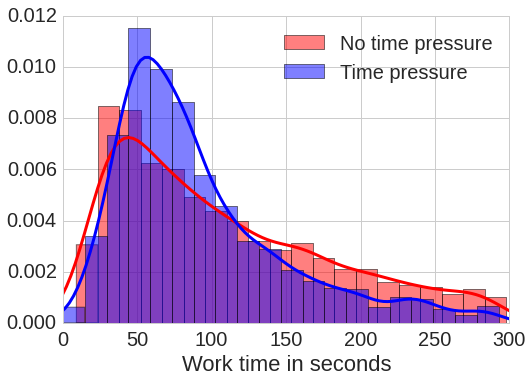
\includegraphics[width=0.4\textwidth]{img/answering_time_distribution}
	\caption{Distribution of answering times for experiments with and without time pressure}
	\label{fig:answering_time_distribution}
\end{figure}

To estimate the quality of answers, we took a sample of 100 questions and repeated the answer rating experiment on this data.
Each answer was judged by 3 different workers (without time pressure), and their scores were averaged.
Figure \ref{fig:average_score} displays the plot with average score for answers from different sources.
Quite surprisingly the quality of collected answers turned out be comparable to those of CQA website users.
Average rating of answers produced by the winning TREC LiveQA system is also pretty close to human answers.
Finally, as expected, time pressure had its negative effect on the quality, however it is still significantly better than quality of an average top 10 QA system.

\begin{figure}[h]
	\centering
	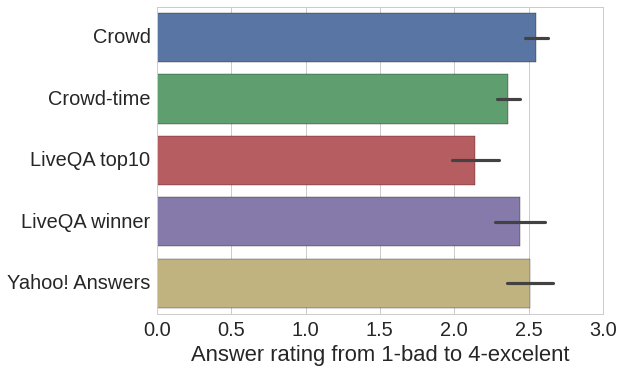
\includegraphics[width=0.4\textwidth]{img/average_score}
	\caption{Average scores of different types of answers to Yahoo! Answers questions}
	\label{fig:average_score}
\end{figure}

\begin{figure}[h]
	\centering
	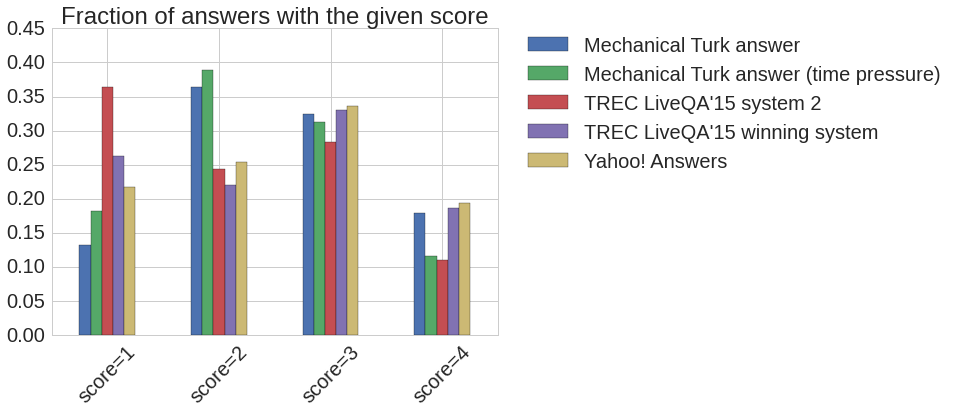
\includegraphics[width=0.4\textwidth]{img/scores_distribution}
	\caption{Distribution of scores for different types of answers to Yahoo! Answers questions}
	\label{fig:scores_distribution}
\end{figure}


Analysis of the score distribution (Figure \ref{fig:scores_distribution}) sheds some light on the nature of the problems with automatic and human answers. The automatic systems generate non-relevant answers ($score=1$) more often than human. Typically this is either fails to retrieve relevant information or distinguish between useful and non-useful answer candidates.
However, by having a larger information store, e.g. world wide web, question answering systems can often find a perfect answer ($score=4$), while crowd workers tend to give generally useful responses ($score=2,3$).

This analysis suggests that regular people can quickly give a reasonable answer to CQA questions.
Of course, some user questions require a certain expertise, which a random crowd worker might not possess.
One idea to tackle this challenge is to design a QA support system, which a worker can use in order to find some additional information.
For example, in our experiment we let workers use web search to find answers, if they were unfamiliar with the topic, and more efficient interfaces are definitely possible.
%Another idea, proposed in \newcite{braunstain2016supporting}, is to automatically retrieve statements and phrases from authoritative sources, that will support the provided answers.

Overall, the results of our study are encouraging, but there are a number of questions, that need to be addressed in order to build an efficient real-time human-computer QA system, which we leave to future work.
For example, such a system needs to scale well to large number and velocity of user questions, which requires an efficient crowd gathering and job assignment components \cite{bernstein2011crowds}.
One potential approach to scalability is selective crowdsourcing, i.e. a system consult the crowd only if it doesn't believe it has a good candidate or it cannot decide between a couple good answers, e.g. based on its internal quality scores.
A real QA system should also use the crowd data as a feedback loop and improve its performance over time, e.g. judged answers should be used to adjust the answer selection model, and answers generated by the crowd should be saved into an archive and reused for future questions.

%An interesting question that we also leave for future work is how an automatic question answering system can put a human in the loop to improve the performance, and how it can utilize different kinds of data a user can quickly produce to be able to generate a reasonable answer while maintaining a near real-time response.
%An automated system, that includes crowdsourcing needs to deal with the above mentioned trustworthiness issues.
%A user, who receives an answer from an expert system will probably trust it more, than if the answer is provided by a random stranger on the internet.


\section{Related Work}
\label{sec:related_work}

Using the wisdom of a crowd to help users satisfy their information needs has been studied before in the literature.
\newcite{bernstein2012direct} explored the use of crowdsourcing for offline preparation of answers to tail search queries.
In this work log mining techniques were used to identify potential question-answer fragment pairs, which were then processed by the crowd to generate the final answer.
This offline procedure allows a search engine to increase the coverage of direct answers to user questions.
In our work, however, the focus is on online question answering, which requires fast responses to the user, who is unlikely to wait more than a minute.
Another related work is targeting a different domain, namely SQL queries.
The CrowdDB system \cite{franklin2011crowddb} is an SQL-like processing system for queries, that cannot be answered by machines only.
In CrowdDB human input is used to collect missing data, perform computationally difficult functions or matching against the query.
In \newcite{aydin2014crowdsourcing} authors explored efficient ways to combine human input for multiple choice questions from the ``Who wants to be a millionaire?'' TV show.
In this scenario going with the majority for complex questions isn't effective, and certain answerer confidence weighting schemas can improve the results.  

Using crowdsourcing for relevance judgments has been studied extensively in the information retrieval community, e.g. \cite{Alonso:2008:CRE:1480506.1480508,alonso2011design,grady2010crowdsourcing} to name a few.
The focus in these works is on document relevance, and the quality of crowdsourced judgments.
Whereas in our paper we are investigating the ability of a crowd to quickly assess the quality of the answers, so a QA system could use this data as a signal.

Crowdsourcing is usually associated with offline data collection, which requires significant amount of time.
Its application to (near) real-time scenarios poses certain additional challenges.
\newcite{bernstein2011crowds} introduced the retainer model for recruiting synchronous crowds for interactive real-time tasks and showed their effectiveness on the best single image and creative generation tasks.
We are planning to build on these ideas and integrate a crowd into a real-time question answering system.
The work of \newcite{Lasecki:2013:CCC:2501988.2502057} showed how multiple workers can sit behind a conversational agent named Chorus, where human input is used to propose and vote on responses. 
Another use of a crowd for maintaining a dialog is presented in \newcite{Bessho:2012:DSU:2392800.2392841}, who let the crowd handle difficult cases, when a system was not able to automatically retrieve a good response from the database of twitter data.
In this paper, we focus on a single part of the human-computer dialog, i.e. question answering, which requires a system to provide some useful information in a response to the user.


\section{Conclusion}
\label{sec:conclusion}

We explored the potential usefulness of crowdsourcing for near real-time question answering by either directly collecting answers from the crowd, or using the crowdsourced judgments to quickly validate automated answers.
Our initial results showed that crowd workers are capable of validating a small set of answer candidates within a minute time limit, which could be potentially incorporated into an automatic QA system for answer validation and reranking (RQ1).
In addition, one minute seems to be enough for a crowd to generate a fair or good response to most real questions drawn from a CQA site, which can be useful in case a QA system didn't have good candidates in the first place (RQ2).
Finally, we compared crowdsourced answers with original Yahoo! Answers responses, and the responses of purely automated LiveQA'15 systems (RQ3).
The quality of such answers on average turned out to be comparable to the original Yahoo! Answers responses, and even with time pressure, crowdsourcing could potentially be useful to complement or augment automatic systems.

%\section*{Acknowledgments}
%If any...

\bibliography{naaclhlt2016}
\bibliographystyle{naaclhlt2016}


\end{document}
